\documentclass[
	fontsize=10pt, % Base font size
	twoside=false, % Use different layouts for even and odd pages (in particular, if twoside=true, the margin column will be always on the outside)
	%open=any, % If twoside=true, uncomment this to force new chapters to start on any page, not only on right (odd) pages
	%chapterprefix=true, % Uncomment to use the word "Chapter" before chapter numbers everywhere they appear
	%chapterentrydots=true, % Uncomment to output dots from the chapter name to the page number in the table of contents
	numbers=noenddot, % Comment to output dots after chapter numbers; the most common values for this option are: enddot, noenddot and auto (see the KOMAScript documentation for an in-depth explanation)
	%draft=true, % If uncommented, rulers will be added in the header and footer
	%overfullrule=true, % If uncommented, overly long lines will be marked by a black box; useful for correcting spacing problems
]{kaohandt}

% Choose the language
\usepackage[english]{babel} % Load characters and hyphenation
\usepackage[english=british]{csquotes}	% English quotes

% Load the bibliography package
\usepackage{styles/kaobiblio}
\addbibresource{main.bib} % Bibliography file

% Load the package for hyperreferences
\usepackage{styles/kaorefs}

% Set the paths where to look for images
\usepackage{subcaption}
\graphicspath{{examples/report/img/}{img/}}

\begin{document}

\title{Operation T-REx}
\author[FM]{Federico Marotta}
\date{December 2019}
\maketitle

\chapter{Introduction}

\section{Le logiciel libre}

Au cours des quelques décennies précédentes, le numérique s'est développé pour intégrer et assister la plupart
des domaines de recherche, des secteurs industriels, ainsi que des aspects de nos vies. Son champ est
aujourd'hui très vaste et connaît en son sein de nombreuses dynamiques différentes ayant un impact sur ses
domaines d'applications, parmi lesquelles celle du logiciel libre.

En essence, les logiciels, applications, services numériques et autres programmes sont des ensembles
d'instructions compréhensibles par un ordinateur et lui indiquant comment utiliser ses ressources afin de
réaliser un certain nombre de tâches. Pour être utilisables par un ordinateur, ces instructions doivent être
formulées en "code machine", un langage souvent représenté en binaire et extrêmement difficile à manipuler par
les humains, même les plus spécialisés, aussi bien en ce qui concerne son écriture que sa compréhension. C'est
pourquoi lors de la création d'un logiciel, les développeurs décrivent d'abord le comportement souhaité dans
un autre langage, textuel et raisonnablement maîtrisable pour un être humain spécialisé, que l'on appelle un
"langage de programmation". Cette description textuelle du logiciel est ce que l'on appelle son "code source",
il est ensuite traduit en code machine par un autre programme (généralement appelé un "compilateur") avant
d'être livré aux personnes souhaitant utiliser le logiciel.

Pour utiliser un logiciel, nous n'avons donc besoin que de son code machine, mais c'est seulement en lisant
son code \emph{source} que l'on peut vraisemblablement comprendre son fonctionnement, corriger ses éventuelles
erreurs, l'adapter à d'autres besoins, vérifier la présence de comportements malveillants, etc. La question de
rendre publiquement disponible le code source d'un logiciel est un enjeu faisant souvent intervenir plusieurs
intérêts divergents, allant de la transparence du fonctionnement de certains services et leur gestion
démocratique au secret industriel.

L'expression "logiciel libre" désigne en français un logiciel disponible publiquement et gratuitement dont le
code source est lui aussi disponible publiquement et gratuitement, ainsi que sa modification et sa
redistribution par toutes et tous. Cette expression désigne aussi et surtout un mouvement visant à développer
la part de logiciel libre dans le numérique, un mouvement dans lequel se développe toute une culture, des
pratiques, des fondations et des événements internationaux. L'expression équivalente anglaise, "\en{Free and
Open Source Software}" (FOSS) est souvent utilisée dans les références citées dans ce mémoire.

\section{Mon parcours personnel}

Étant issu d'une formation d'ingénieur spécialisée en informatique, mon domaine d'expertise se situe
principalement dans le numérique, et en particulier dans le développement logiciel. Mon parcours m'a
rapidement amené au logiciel libre, notamment via les technologies utilisées au sein de mon école d'ingénieur,
l'\gls{epita}, mais surtout via mon implication pendant mes études dans des associations comme
Prologin\sidenote{\url{https://prologin.org}} et GConfs\sidenote{\url{https://gconfs.fr}} : l'une organisant
un concours francophone d'algorithmique ainsi que des stages d'initiation à l'informatique pour
lycéennes\sidenote{\url{https://girlscancode.fr/}}, l'autre œuvrant au partage de connaissance entre pairs en
organisant des conférences par les élèves et pour les élèves au sein de l'école. Ces deux associations ont
produit des sites web ainsi que de nombreux outils informatiques, tous sur le principe du logiciel libre, ce
qui a beaucoup contribué aux échanges avec leurs publiques cibles en permettant à tous de participer,
commenter et améliorer les outils développés, en plus d'accroitre la transparence de leurs structures.
Plusieurs des outils développés par ces associations ont d'ailleurs été réutilisés dans d'autres contextes par
d'autres personnes qui leurs sont externes. Cette implication dans le mouvement du logiciel libre m'a aussi
amené à assister régulièrement au \gls{fosdem}\sidenote{\url{https://fosdem.org}}, la conférence principale du
logiciel libre en Europe, aussi bien l'occasion de s'informer sur l'évolution des nombreuses communautés du
logiciel libre qu'un prétexte pour y retrouver de vieilles connaissances lors d'un week-end à Bruxelles.

Mon parcours s'est ensuite enrichi d'une expérience dans l'enseignement lorsque j'ai rejoint pendant ma
cinquième et dernière année à l'\gls{epita} la petite équipe des "assistants", qui encadre l'enseignement de
la principale matière informatique pour les étudiants de troisième année. J'ai écrit et évalué au sein de
cette équipe des sujets de travaux pratique et encadré de nombreuses séances de travail sur ordinateur, ce qui
a développé chez moi une forte appétence pour l'enseignement. J'ai souhaité explorer cette appétence après la
fin de mes études lors d'un service civique au collège et lycée Jean Monnet de Strasbourg, où j'y ai donné des
cours de soutient. Ayant confirmé mon intérêt pour cette voie professionnelle, je suis revenu à l'\gls{epita}
pour y devenir enseignant des matières informatiques, à l'occasion de l'ouverture de son nouveau campus à
Strasbourg.

Enfin, de nombreuses discussions avec des amis chercheurs et passionnés de méthodologie scientifique, ainsi
qu'une tentative personnelle pour me familiariser avec la recherche en éducation, m'ont poussé à entreprendre
une formation m'aidant d'une part à développer mes connaissances en éducation, et me fournissant d'autre part
une introduction à la recherche scientifique, tout en exploitant mes acquis en informatique. C'est ainsi que
je me suis inscrit au Master SYNVA et que je cherche, à travers ce mémoire, à explorer et contribuer à la
recherche touchant ces domaines de l'informatique, de l'enseignement, ainsi que de la libération de la
connaissance et de l'information.

\section{Les projets de logiciel libre dans l'enseignement de l'informatique}

La pédagogie de projet est une méthode d'enseignement qui consiste à inviter les apprenants à appliquer leurs
connaissances et à en acquérir de nouvelles au travers d'un projet plus ou moins concret et imitant plus ou
moins fidèlement une situation réelle. Réalisé soit individuellement soit en groupe, les projets aboutissent
généralement à une production évaluée par l'enseignant, parfois au travers d'une présentation donnée par les
apprenants. L'efficacité de cette méthode a fait l'objet de nombreuses recherches au cours des années
précédentes. Plusieurs méta-analyses concluent que cette méthode a des effets mesurables, positifs et
importants sur les résultats académiques des apprenants en sciences sociales et en sciences naturelles
\sideparencite{pbl-2019, pbl-2018}.

Les projets proposés aux étudiants sont le plus souvent factices, imaginés par les enseignants dans le seul
but de servir d'exercice. Utiliser au contraire des projets réels, qui ne cessent pas d'exister après la fin
de la séquence pédagogique, sur lesquels faire travailler les étudiants donne des résultats encore meilleurs,
mais est aussi plus difficile et incertain à encadrer pour les enseignants \sideparencite{real-pbl-2010,
real-pbl-2004}. Il est notamment très difficile pour l'enseignant de prévoir à l'avance les problèmes que les
apprenants risquent de rencontrer, c'est pourquoi d'autres efforts dans cette direction ont tenté un
compromis, consistant à créer des projets de logiciel libre aussi proches des situations réelles que possible,
mais dédiés à l'éducation \sideparencite{oss-edu-2008}. Les projets en question ne sont cependant plus
accessibles aujourd'hui, une explication possible à leur disparition étant leur portée réduite à l'éducation
et l'absence d'une communauté persistante autour d'eux.

Bien qu'elles soient plutôt rares, quelques initiatives existent aussi pour enseigner spécifiquement les
pratiques du logiciel libre dans l'éducation supérieur et la formation tout au long de la vie. Certaines sont
des initiatives venant des communautés du logiciel libre, comme le \en{Professional Certificate in Open Source
Software Development, Linux and Git}%
\sidenote{\url{https://www.edx.org/professional-certificate/linuxfoundationx-open-source-software-development-linux-and-git}}
de la \en{Linux Foundation}, et en particulier la première séquence : \en{Open Source Software Development:
Linux for Developers}%
\sidenote{\url{https://www.edx.org/course/open-source-software-development-linux-for-developers}} ; ou les
séminaires de l'\en{open source initiative}\sidenote{\url{https://opensource.org/osi-open-source-education}}.
Enfin, certaines universités proposent des cursus en informatique ayant des éléments visant spécifiquement les
pratiques du logiciel libre, c'est le cas notamment de l'Université de l'État de Caroline du Nord aux
États-Unis, qui a expérimenté plusieurs façons d'inclure la contribution aux projets de logiciel libre dans
leurs cursus d'informatique \sideparencite{oss-edu-2008, oss-edu-2007} ; mais aussi de l'université de Calais
qui propose actuellement un "Master Informatique - Ingénierie du logiciel libre"%
\sidenote{\url{https://www.univ-littoral.fr/formation/offre-de-formation/masters/master-informatique-ingenierie-du-logiciel-libre/}},
sous la forme d'une formation en alternance.

\section{Data}
\labsec{data}

The Genotype-Tissue Expression (GTEx) project \sidecite{Lonsdale2013a} 
aims to characterise gene expression and regulation for 54 human healthy 
tissues across nearly 1000 people. While the results of the analyses are 
open-access, in order to gain access to the raw data about the DNA and 
the gene expression of the individuals, it is necessary to go through a 
long bureaucratic procedure.

Another source of data was the Ensembl project (release 75), 
\sidecite[-1.55cm]{Zerbino2018} which was used to obtain the coordinates 
of the regulatory regions for each gene. Regulatory regions are 
particular positions around a gene where transcription factors can bind; 
from there, these transcription factors exert a control on gene 
expression.\sidenote{In this project, I considered 141 genes of a 
particular type of blood cells, for 95 individuals. Each gene is 
associated to about 10 regulatory regions on average.} Each 
transcription factor recognises a specific sequence of DNA, therefore it 
is possible to compute the affinity of a factor for a given region. The 
total binding affinity (TBA) \sidecite[-3.85cm]{Molineris2011a} is one 
of the possible affinity measures.\sidenote[][]{The TBA is also 
related to the name of this project, T-REx: indeed, the goal is to 
estimate the TBA-Regulated Expression.}

Gene expression in GTEx was measured with a technique called 
RNA-sequencing, which returns, for each gene and each individual, the 
RPKM, \sidecite[-4.6cm]{Mortazavi2008} which is the number of sequencing 
reads normalised by the length of the gene and by the total number of 
reads.

%\begin{figure}[H]
\begin{figure}[H]
  \begin{subfigure}{\textwidth}
	\centering
	\caption{}
%	\caption{Histogram and normal Q\babelhyphen{nobreak}Q plot of the 
%expression of a randomly selected gene called BID. In the histogram, the 
%brown dashed line indicates the mean, while the dotted lines indicate 
%plus and minus one standard deviation. In the Q\babelhyphen{nobreak}Q 
%plot, each point represents an individual.}
	\labfig{distrexpr}
	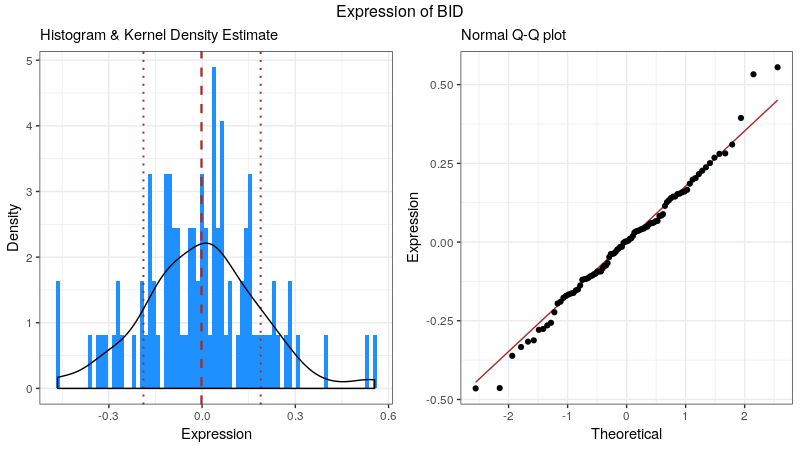
\includegraphics[height=4.8cm,width=.8\textwidth,keepaspectratio=false]{bid_expr}
  \end{subfigure}
%\end{figure}

  \begin{subfigure}{\textwidth}
%\begin{figure}[t]
    \centering
    \caption{}
% 	\caption{Scree plot and biplot of 
% the \textasciitilde800 affinities for the gene BID. In the biplot, each 
% label corresponds to an individual.}
    \labfig{pcatba}
    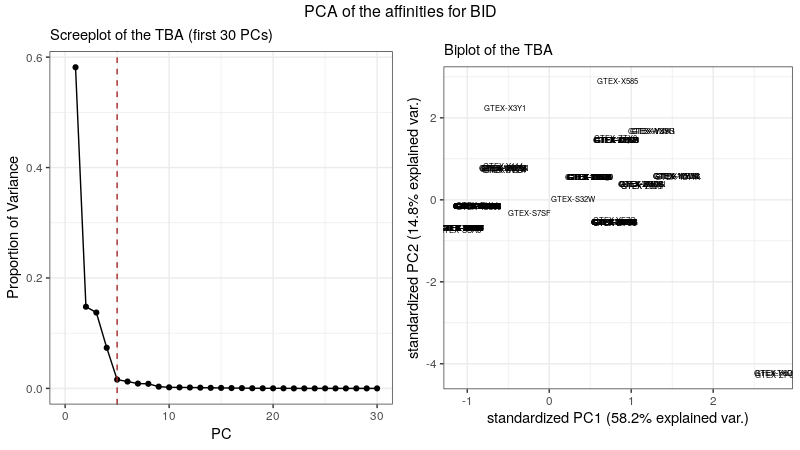
\includegraphics[height=4.8cm,width=.8\textwidth,keepaspectratio=false]{bid_tba}
  \end{subfigure}
% \end{figure}
  \caption{(a): Histogram and normal Q\babelhyphen{nobreak}Q plot of the 
expression of a randomly selected gene called BID. In the histogram, the 
brown dashed line indicates the mean, while the dotted lines indicate 
plus and minus one standard deviation. In the Q\babelhyphen{nobreak}Q 
plot, each point represents an individual. (b): Scree plot and biplot of 
the \textasciitilde800 affinities for the gene BID. In the biplot, each 
label corresponds to an individual.}
  \labfig{expl}
\end{figure}

The expression was preprocessed as recommended by the Stephen's 
Lab.\sidenote[][*7]{\url{http://stephenslab.github.io/gtex-eqtls/analysis/20170515\_RNASeq\_Analysis.html}} 
In summary, I applied a quantile normalisation to make sure that the 
distribution of our response variable was normal, and then I obtained 
the residuals of a linear model 
$Y~\sim~SEX+PEER\_FA+POPULATION+PLATFORM$, so as to disregard the 
effects of these covariates on the expression. The final result can be 
seen in \reffig{distrexpr}.

The genotypes were also obtained with a sequencing technique and were 
provided in VCF format. \sidecite[-3.2cm]{Danecek2011} I 
used a software called 
\nohyphens{VCF\textunderscore\nobreak\hspace{0pt}rider}\sidenote[][*3]{\url{https://github.com/vodkatad/vcf\_rider}} 
to compute the total binding affinity of each transcription factor for 
each regulatory region associated to a gene (the total number of 
transcription factors is about 800). \reffig{pcatba} reports the PCA of 
the TBA for the gene BID.

\pagelayout{wide}
\setchapterstyle{kao}
\chapter{Résultats}

\todo[inline]{%
    TODO : analyser hasContrib et rédiger. Voir aussi s'il n'est pas pertinent de retirer tous les projets
    ayant moins de deux contributeurs récents (les résultats sont nettement plus positifs de cette façon :
    \texttt{hasContrib} donne deux moyennes très différentes et le $r^2$ des régressions linéaires augmente
    beaucoup)%
}

\begin{tabular}{cc}
    \begin{tabular}{ll}
 & hasContrib \\
count & 27619 \\
unique & 2 \\
top & no \\
freq & 23740 \\
\end{tabular}
 &
    \begin{tabular}{lr}
 & newContributorCount \\
count & 60966.000000 \\
mean & 0.522209 \\
std & 1.663200 \\
min & 0.000000 \\
25\% & 0.000000 \\
50\% & 0.000000 \\
75\% & 1.000000 \\
max & 130.000000 \\
\end{tabular}

    \\
    \begin{tabular}{lr}
 & \textbf{recentContributorCount} \\
count & 60966.000000 \\
mean & 3.246268 \\
std & 6.983897 \\
min & 2.000000 \\
25\% & 2.000000 \\
50\% & 2.000000 \\
75\% & 3.000000 \\
max & 688.000000 \\
\end{tabular}
 &
    \begin{tabular}{lr}
 & \textbf{recentCommitCount} \\
count & 60966.00 \\
mean & 61.79 \\
std & 408.96 \\
min & 2.00 \\
25\% & 8.00 \\
50\% & 19.00 \\
75\% & 49.00 \\
max & 36176.00 \\
\end{tabular}

\end{tabular}

\begin{figure}[ht]
    \begin{subfigure}[t]{0.5\textwidth}
        \includesvg[width=\textwidth]{experiment/data_analysis/hasContrib_Count.svg}
        \caption{Nombre de projets avec ou sans instructions de contribution}
    \end{subfigure}%
    \begin{subfigure}[t]{0.5\textwidth}
        \includesvg[width=\textwidth]{experiment/data_analysis/hasContrib_meanNewContributorCount.svg}
        \caption{Moyenne du nombre de nouveaux contributeurs avec ou sans instructions de contribution}
    \end{subfigure}

    \caption{Effet de la présence d'instructions de contribution}
    \label{fig:hasContrib}
\end{figure}

\todo[inline]{%
    Pour vérifier à quel point cette (minuscule) différence de moyenne s'explique effectivement par
    \texttt{hasContrib}, il faudrait faire une one-way ANOVA, mais apparemment il faut que la population de
    base suive une loi normale, ce qui n'est pas du tout le cas, il y a peut être une application du théorème
    central limite qui peut m'aider ?
}

\begin{figure}[ht]
    \centering
    \begin{subfigure}[t]{0.5\textwidth}
        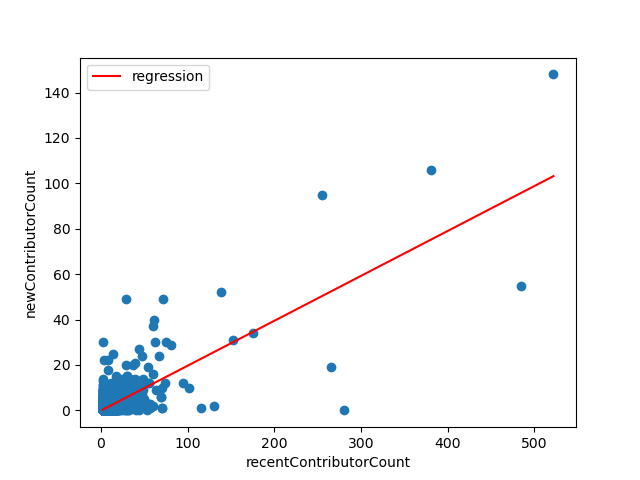
\includegraphics[width=\textwidth]{experiment/data_analysis/recentContributorCountRegression_linearScale.png}
        \caption{Échelle linéaire}
    \end{subfigure}%
    \begin{subfigure}[t]{0.5\textwidth}
        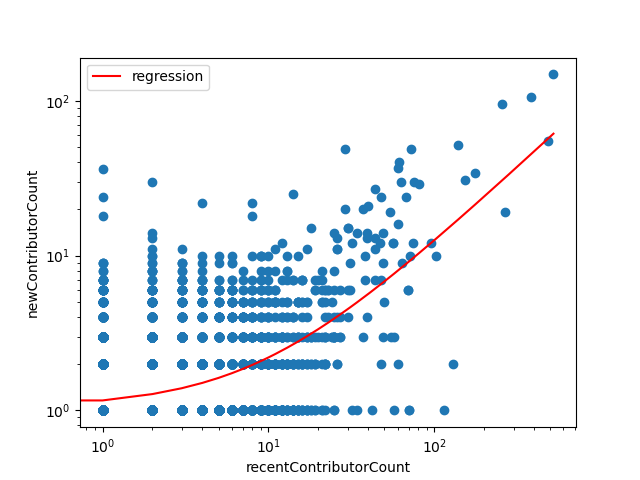
\includegraphics[width=\textwidth]{experiment/data_analysis/recentContributorCountRegression_logScale.png}
        \caption{Échelle logarithmique}
    \end{subfigure}

    $\mathit{newContributorCount} = \mathit{recentContributorCount} * 0.11540180 + 1.04427117$\\($r^2 = 0.28318792$)
    \caption{Nombre de nouveaux contributeurs en fonction du nombre de contributeurs récents uniques}
    \label{fig:contributorCount}
\end{figure}

\begin{figure}[ht]
    \centering
    \begin{subfigure}[t]{0.5\textwidth}
        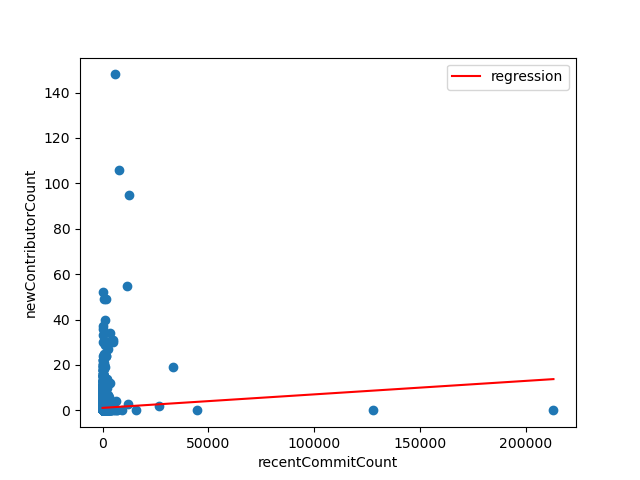
\includegraphics[width=\textwidth]{experiment/data_analysis/recentCommitCountRegression_linearScale.png}
        \caption{Échelle linéaire}
    \end{subfigure}%
    \begin{subfigure}[t]{0.5\textwidth}
        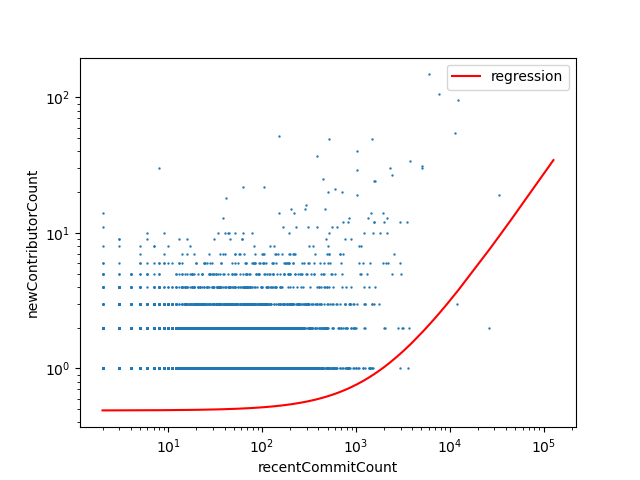
\includegraphics[width=\textwidth]{experiment/data_analysis/recentCommitCountRegression_logScale.png}
        \caption{Échelle logarithmique}
    \end{subfigure}

    $\mathit{newContributorCount} = \mathit{recentCommitCount} \times 0.00026672041 + 0.48979364$\\($r^2 = 0.12749825$)
    \caption{Nombre de nouveaux contributeurs en fonction du nombre de commits récents}
    \label{fig:commitCount}
\end{figure}

\pagelayout{margin}

\chapter{Discussion}

\todo[inline]{%
    Pour hasContrib j'ai utilisé un test de Mann-Whitney, la valeur p est ridiculement petite, ce qui
    apparemment s'expliquerait surtout par la taille de mon jeu de donnée et pas tant par le pouvoir
    explicatif de hasContrib, donc a prendre avec des pincettes, mais il me faudrait une citation si je veux
    vraiment avancer ça.
}


\defbibnote{bibnote}{Here are the references in citation order.\par\bigskip} % Prepend this text to the bibliography
\renewcommand*{\bibfont}{\small}
\printbibliography[title=Bibliography]% , prenote=bibnote]

\end{document}
